% Options for packages loaded elsewhere
\PassOptionsToPackage{unicode}{hyperref}
\PassOptionsToPackage{hyphens}{url}
%
\documentclass[
]{article}
\usepackage{amsmath,amssymb}
\usepackage{lmodern}
\usepackage{iftex}
\ifPDFTeX
  \usepackage[T1]{fontenc}
  \usepackage[utf8]{inputenc}
  \usepackage{textcomp} % provide euro and other symbols
\else % if luatex or xetex
  \usepackage{unicode-math}
  \defaultfontfeatures{Scale=MatchLowercase}
  \defaultfontfeatures[\rmfamily]{Ligatures=TeX,Scale=1}
\fi
% Use upquote if available, for straight quotes in verbatim environments
\IfFileExists{upquote.sty}{\usepackage{upquote}}{}
\IfFileExists{microtype.sty}{% use microtype if available
  \usepackage[]{microtype}
  \UseMicrotypeSet[protrusion]{basicmath} % disable protrusion for tt fonts
}{}
\makeatletter
\@ifundefined{KOMAClassName}{% if non-KOMA class
  \IfFileExists{parskip.sty}{%
    \usepackage{parskip}
  }{% else
    \setlength{\parindent}{0pt}
    \setlength{\parskip}{6pt plus 2pt minus 1pt}}
}{% if KOMA class
  \KOMAoptions{parskip=half}}
\makeatother
\usepackage{xcolor}
\usepackage[margin=1in]{geometry}
\usepackage{graphicx}
\makeatletter
\def\maxwidth{\ifdim\Gin@nat@width>\linewidth\linewidth\else\Gin@nat@width\fi}
\def\maxheight{\ifdim\Gin@nat@height>\textheight\textheight\else\Gin@nat@height\fi}
\makeatother
% Scale images if necessary, so that they will not overflow the page
% margins by default, and it is still possible to overwrite the defaults
% using explicit options in \includegraphics[width, height, ...]{}
\setkeys{Gin}{width=\maxwidth,height=\maxheight,keepaspectratio}
% Set default figure placement to htbp
\makeatletter
\def\fps@figure{htbp}
\makeatother
\setlength{\emergencystretch}{3em} % prevent overfull lines
\providecommand{\tightlist}{%
  \setlength{\itemsep}{0pt}\setlength{\parskip}{0pt}}
\setcounter{secnumdepth}{-\maxdimen} % remove section numbering
\ifLuaTeX
  \usepackage{selnolig}  % disable illegal ligatures
\fi
\IfFileExists{bookmark.sty}{\usepackage{bookmark}}{\usepackage{hyperref}}
\IfFileExists{xurl.sty}{\usepackage{xurl}}{} % add URL line breaks if available
\urlstyle{same} % disable monospaced font for URLs
\hypersetup{
  pdftitle={Simulate disparate impact stats},
  pdfauthor={Max Griswold},
  hidelinks,
  pdfcreator={LaTeX via pandoc}}

\title{Simulate disparate impact stats}
\author{Max Griswold}
\date{2024-01-11}

\begin{document}
\maketitle

\hypertarget{simulate-how-disparate-impact-statistics-can-fail}{%
\section{Simulate how disparate impact statistics can
fail}\label{simulate-how-disparate-impact-statistics-can-fail}}

\hypertarget{max-griswold}{%
\section{Max Griswold}\label{max-griswold}}

\hypertarget{section}{%
\section{1/9/24}\label{section}}

Disparate impact cases require demonstrating if a disparity in outcomes
for a protected class is statistically significant and sufficiently
sized. This project aims to use simulation to show a range of cases
where the conventional statistical rules for determining a disparate
impact -the four-fifths rule and significance rule - can lead to
different conclusions due

This notebook demonstrates a simplified example of how we might conduct
simulations. The setup concerns a landlord determining whether to accept
a tenant's rental application, based on their income and
former-incarceration status. In each of the three scenarios below, the
landlord aims to deny tenancy to applicants based on their race.

To start, I generate data according to the following data generating
process (figure 1). I assume that an applicant's race is correlated both
with their monthly earnings and with the probability of being
formerly-incarcerated. I also assume monthly earnings also depend on
former incarceration status. I assume in each scenario that these three
variables uniquely determine if a landlord

I determined the probability of former incarceration status using data
from \href{https://bjs.ojp.gov/content/pub/pdf/Llgsfp.pdf}{DOJ-OJP},
monthly earnings based off
\href{https://www.census.gov/library/publications/2023/demo/p60-279.html}{Census
income}, and the effect of incarceration status on monthly earnings,
stratified by race, from estimates in
\href{https://scholar.harvard.edu/files/brucewestern/files/racial_inequality_in_employment_and_earnings_after_incarceration.pdf}{Western,
2017}.

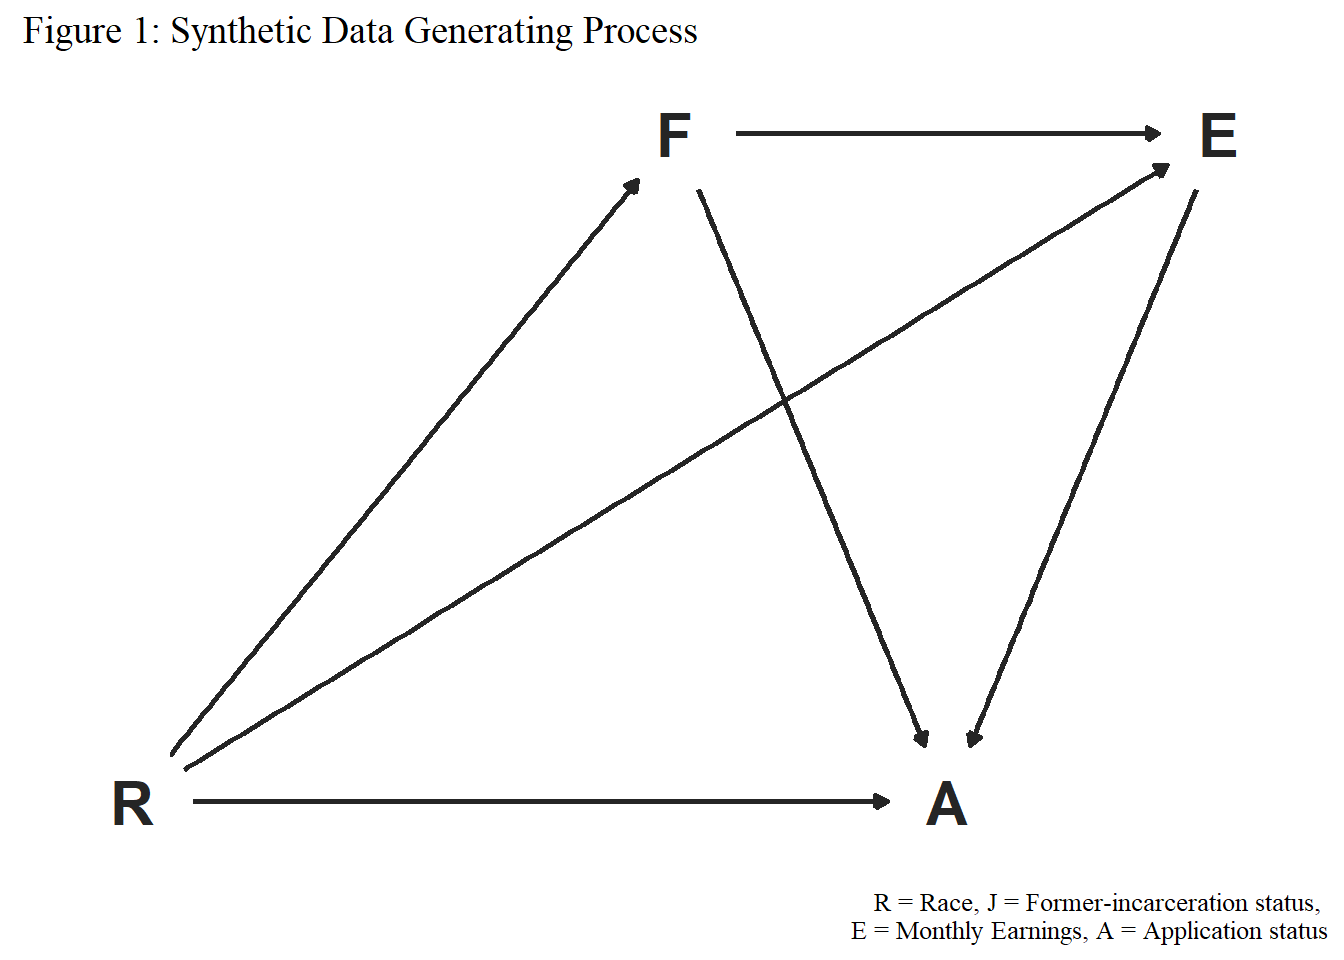
\includegraphics{disparate_impact_synthetic_scenario_example_files/figure-latex/unnamed-chunk-1-1.pdf}

I set up the following decision scenarios for the landlord:

\begin{enumerate}
\def\labelenumi{\arabic{enumi}.}
\tightlist
\item
  The landlord engages in direct discrimination: If the applicant is
  black, they offer a unit to them 25\% less often than a comparable
  white candidate.
\item
  The landlord attempts to obscure their motive by only denying tenancy
  to a fraction of applicants. Every third black applicant they
  encounter, they deny their tenancy 75\% more often.
\item
  The landlord puts more weight on former-incarceration status to decide
  if they deny an applicant tenancy. They choose a probability of
  denying tenancy based on former-incarceration status so they deny
  tenancy to an equal proportion of black-to-white tenants as in the
  first two scenarios.
\end{enumerate}

Across all scenarios, the same ratio of black-to-white applicants are
denied tenancy. I used monte-carlo simulation to generate 500 synthetic
datasets and varied the sample size of applicants between 200 and 4000.

For each simulation and scenario, I regressed a tenant's application
status (accepted or denied) on the tenant's race, former-incarceration
status, and monthly earnings using a binomial regression with a logit
link. This is a routine model used to detect disparate impact
(\href{https://www.law.upenn.edu/live/files/1138-ayresincludedvariablebiaspdf}{Ayres,
2010}; \href{https://5harad.com/papers/included-variable-bias.pdf}{Jung
et al., 2023})

I then obtained the estimated p-value for the beta-coefficient on race
and used the regression equation to calculate an estimate for the ratio
of black-to-white applicants denied tenancy. Finally, I took the mean of
these estimates across simulation iterations.

To meet the standards for disparate impact, the protected class needs to
be selected as an applicant less than 80\% of the time (the four-fifths
rule) and this effect needs to be significant at the 0.05 significance
level. Since we set up the scenarios, we know for a fact that landlords
are discriminating against black applicants 25\% more often than white
applicants. However, can the models detect this effect?

Figure 2 displays the estimated rate at which black applicants are
selected for a unit compared to white applicants. For scenario 1 and 2,
the model is able to detect a disparity of roughly 70\%. For scenario 3,
the estimated disparity is close to 100\%. While scenario 1 and 2 are
able to meet the four-fifths rule, all scenarios underestimate the true
disparity. This can be seen by examining the data generating process.
Since the models include controls, the effects of race in these models
will not estimate the mediating effect of race on earnings and
former-incarceration status. Accordingly, all estimates are unable to
detect the true disparity observed in the outcome. Increasing sample
size does not improve the ability of the models to detect the true
disparity.

\includegraphics{disparate_impact_synthetic_scenario_example_files/figure-latex/ratio plot-1.pdf}

Additionally, the estimating equations vary substantially in terms of
detecting effects at a 0.05 significance level. Figure 3 below displays
the average estimated p-value by scenario and sample sizes. Scenario 1
is identified by the model once there's a sample size of 1000 Scenario
2, which is more variable in how the the landlord makes a discriminatory
decision, unsurprisingly requires a larger sample size to detect the
effect, needing a minimum sample size of 1200.

However, in scenario 3, the model is unable to detect a significant
effect at any sample size. This scenario is the canonical case where
disparate impact tests would be most useful since the landlord's
decision-making did not depend on race per se (i.e.~no intent) but led
to a disparate impact. This result should be unsurprising based on the
data generating process above (since the model controls for both
earnings and former incarceration status, there is no possibility for
the race variable to generate an effect).

This result also aligns with existing scholarship which criticizes the
use of examining the treatment effect of race as a measure of
discrimination. (Kohler-Hausmann,
2019){[}\url{https://scholarlycommons.law.northwestern.edu/cgi/viewcontent.cgi?article=1374\&context=nulr}{]};
(Heckman,
1998){[}\url{https://www.aeaweb.org/articles?id=10.1257/jep.12.2.101}{]}.
Since the model controls for variables causally related to race, which
is a routine practice done during disparate impact analyses, the model
removes many of the factors causing discriminatory impacts due to race.
Previous scholars have described this as the ``included variable bias''
(\href{https://www.law.upenn.edu/live/files/1138-ayresincludedvariablebiaspdf}{Ayres,
2010}; \href{https://5harad.com/papers/included-variable-bias.pdf}{Jung
et al., 2023}). In particular Jung et al., 2023 demonstrates that by
weighting averages of differences across groups balanced by control
covariates, it might be possible to identify the actual disparity.

However, as Figure 2 shows, this could introduce a new problem: smaller
sample sizes, making it less likely to meet the statistical significance
rule. Since the Jung approach requires stratifying differences and
creating a unitary measure of risk, a larger sample size would be needed
to identify disparities. One potential solution to this suggested by
previous work, is that courts should use probabilities of detecting an
effect in place of statistical significance (Miao and Gastwirth,
2013){[}\url{https://academic.oup.com/lpr/article/12/1/37/925237\#15990473}{]}..
But this would require determining study power, which might not be
possible to due a lack of reliable previous studies and the limiations
of determinig statistical power after collecting data (Dziak, Dierker,
and Abar,
2020){[}\url{https://www.ncbi.nlm.nih.gov/pmc/articles/PMC7286546/}{]}.

Less discussed by previous literature is the idea that data used to
determine the existence of disparate impacts exists might contain
included-variable bias within the data itself. For example, (Knox, Lowe,
and Mummolo,
2020){[}\url{https://www.cambridge.org/core/journals/american-political-science-review/article/administrative-records-mask-racially-biased-policing/66BC0F9998543868BB20F241796B79B8?utm_source=hootsuite\&utm_medium=twitter\&utm_term=\&utm_content=FirstView\&utm_campaign=PS}{]}
discusses how administrative records mask biases embedded into the
dataset itself. Examining arrest records, they find that estimates of
racial discrimination are understimates of the true effect since it is
impossible to recover a necessary variable: citizens observed by race
but not arrested.

In effect, this is an example of an included variable bias since the
dataset contains a variable correlated with race that is implicitly
controlled (that is, data on arrests is conditional on being observed).
Accordingly, the approach of Jung et al., might be impossible to perform
using critical datasets examined within disparate impact cases. Knox,
Lowe, and Mummolo also propose an alternative way to detect a
discriminatory difference by bounding the effect using assumptions on
discriminatory intent or by using gold-standard data which does not
contain racial biases and can identify an estimate for the missing
``included-variable''. In the instance of bounding effects, this
procedure may lead to finding effect ranges which no longer meet the
four-fifths standard.

With this research in mind, this study will aim to construct synthetic
datasets which contain properties matching datasets used in existing
cases on disparate impact. Through the use of these synthetic datasets,
we will examine how often current procedures are able to recover known
disparate impacts and meet the rule standards, given increased sample
sizes or modifications to model specifications addressing
included-variable bias. Additionally, we will explore the extent to
which it is possible to apply potential solutions to included-variable
bias, since this is essential bias to resolve given the purpose of
disparate impact cases (e.g., scenario 3 above). We will also assess how
the use of these tests may modify the ability to meet the two rule
standards of disparate impact testing: the four-fifths rule and the
statistical significance standard.

\includegraphics{disparate_impact_synthetic_scenario_example_files/figure-latex/pvalue v. sample-1.pdf}

\end{document}
